\section{Audit results: lens mismatch, localization, and staging}
\label{sec:results-audits}

We now treat the SPT2018 likelihood and the SPT D1 likelihood as two \emph{lenses} on (nearly) the same sky field. The central question is whether packaged outputs are stable under swapping these lenses. Following \cref{eq:dchi_def}, we quantify stability via directional held-out mismatch statistics and then localize the mismatch by spectrum and multipole.

\subsection{Directional mismatch is large and asymmetric}
Table~\ref{tab:audit-summary} summarizes the directional cross-lens audit statistics for both the \emph{unprofiled} audit (evaluating each lens at the other lens's best-fit point) and the \emph{profiled} audit (re-optimizing a tractable subset of the test lens's nuisance parameters; \cref{sec:profiled-audit}). Two qualitative features are immediate:
\begin{enumerate}[leftmargin=*, itemsep=2pt]
  \item \textbf{Mismatch is directional.} The values of $\dchi_{B|A}$ and $\dchi_{A|B}$ differ substantially, indicating that route mismatch is not symmetric across the two lenses.
  \item \textbf{Mismatch is large even after profiling.} Profiling reduces sensitivity to purely lens-specific nuisance packaging, but does not eliminate the held-out failure, indicating that the mismatch is not solely a matter of nuisance retuning.
\end{enumerate}

\begin{table}[t]
  \centering
  \caption{Directional cross-lens audit summary for SPT2018 vs SPT D1, with and without common-staging. The unprofiled audit uses direct evaluation of the test lens at the train lens's best-fit point; the profiled audit re-optimizes a tractable subset of test-lens nuisance parameters at fixed shared parameters (\cref{sec:profiled-audit}). ``Common-staging'' restricts the D1 lens to the SPT2018 multipole support (\cref{sec:common-staging}).}
  \label{tab:audit-summary}
  \resizebox{\linewidth}{!}{\begin{tabular}{@{}l l r r@{}}
\toprule
Audit scope & Variant & $\dchi_{\mathrm{D1}|2018}$ & $\dchi_{2018|\mathrm{D1}}$ \\
\midrule
SPT only, fixed spectra & nuisance-profiled & 849.63 & 414.39 \\
 & + support cut & 837.15 & 415.79 \\
\addlinespace
SPT + DESI & baseline & 488.30 & 79.13 \\
 & + support cut & 486.61 & 80.52 \\
\addlinespace
Full CMB + DESI & baseline (multistart) & 62.59 & 23.17 \\
 & baseline (warm start) & 62.39 & 23.19 \\
 & + support cut & 64.62 & 23.39 \\
 & $-$ SPT $\tau$ prior & 61.28 & 23.11 \\
 & + CLASS precision & 61.39 & 23.08 \\
\bottomrule
\end{tabular}
}
\end{table}

\subsection{Localization points to TT high-$\ell$ structure in the overlap region}
To make the mismatch actionable, we localize $\dchi$ by decomposing it into contributions grouped by spectrum type and multipole ranges. Figure~\ref{fig:profiled-localization} shows the resulting localization heatmaps for the \emph{profiled} audit in both directions. The dominant contributions arise from TT at high multipoles (notably the $\ell\sim 2000$--$3000$ range), while TE/EE contributions are comparatively small.
Because high-$\ell$ TT is foreground- and calibration-sensitive, this localization should be read as identifying where the \emph{packaged likelihood objects} disagree (e.g., foreground modeling, calibration/beam/transfer-function conventions, or covariance structure), not as a map-level diagnosis of the sky.

A key observation is that these multipoles lie well \emph{inside} the overlap region of the two SPT lenses. In other words, the mismatch is not primarily driven by the fact that D1 extends to lower $\ell$ in TT or to higher $\ell$ in TE/EE. Rather, the held-out failure is concentrated in TT structure that both lenses nominally cover. This localization supports interpreting the ``curious shift'' highlighted in \cite{arxiv2601_16277} as a packaging stability failure tied to how the two lenses compress and model the same underlying sky information.

\begin{figure}[t]
  \centering
  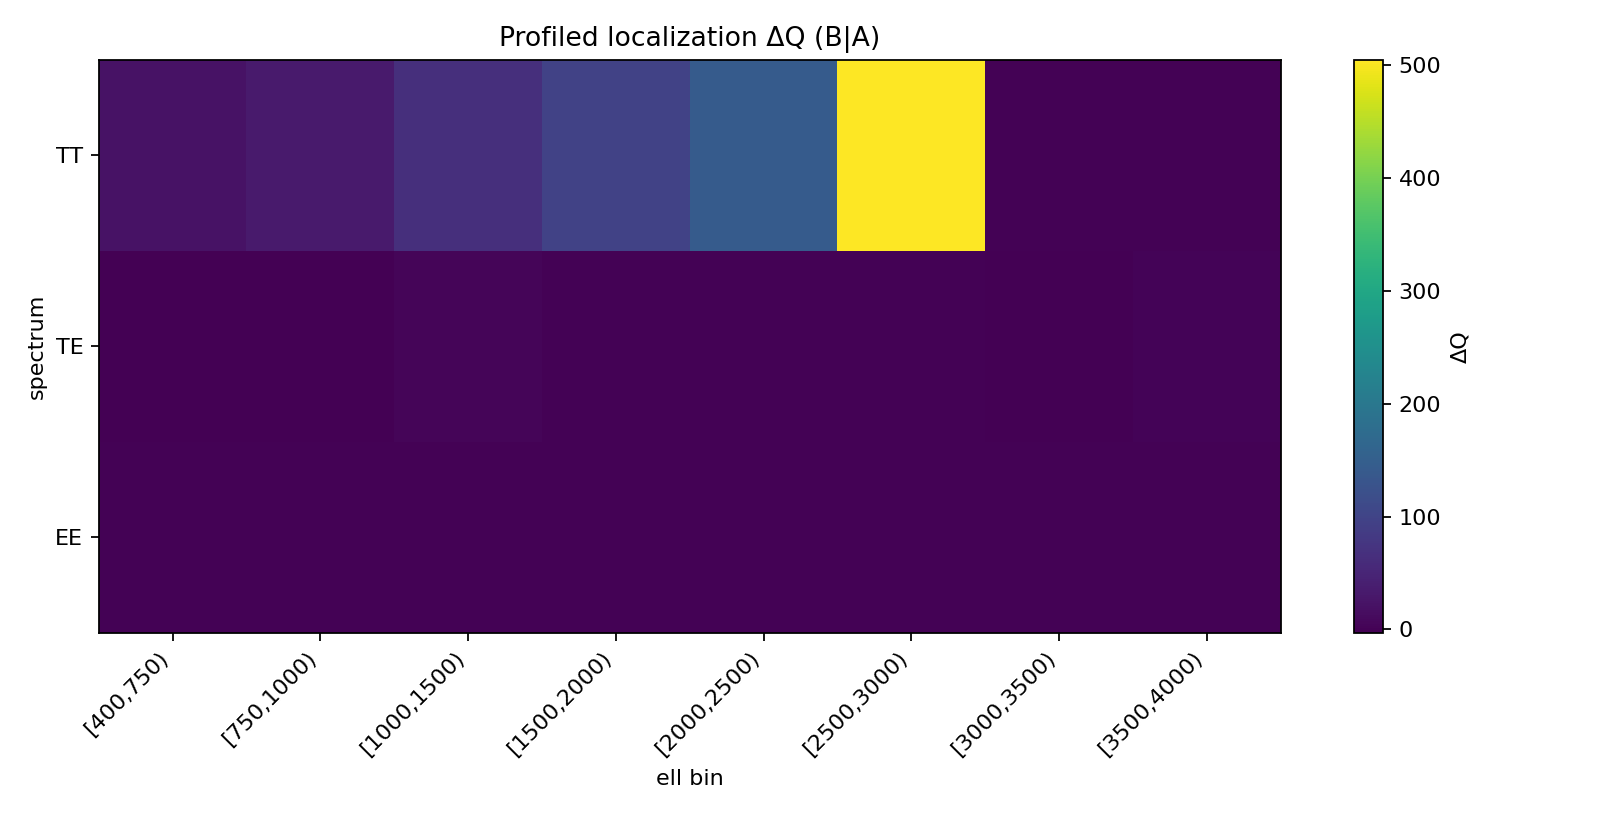
\includegraphics[width=0.49\linewidth]{figures/fig_profiled_localization_B_given_A.png}
  \hfill
  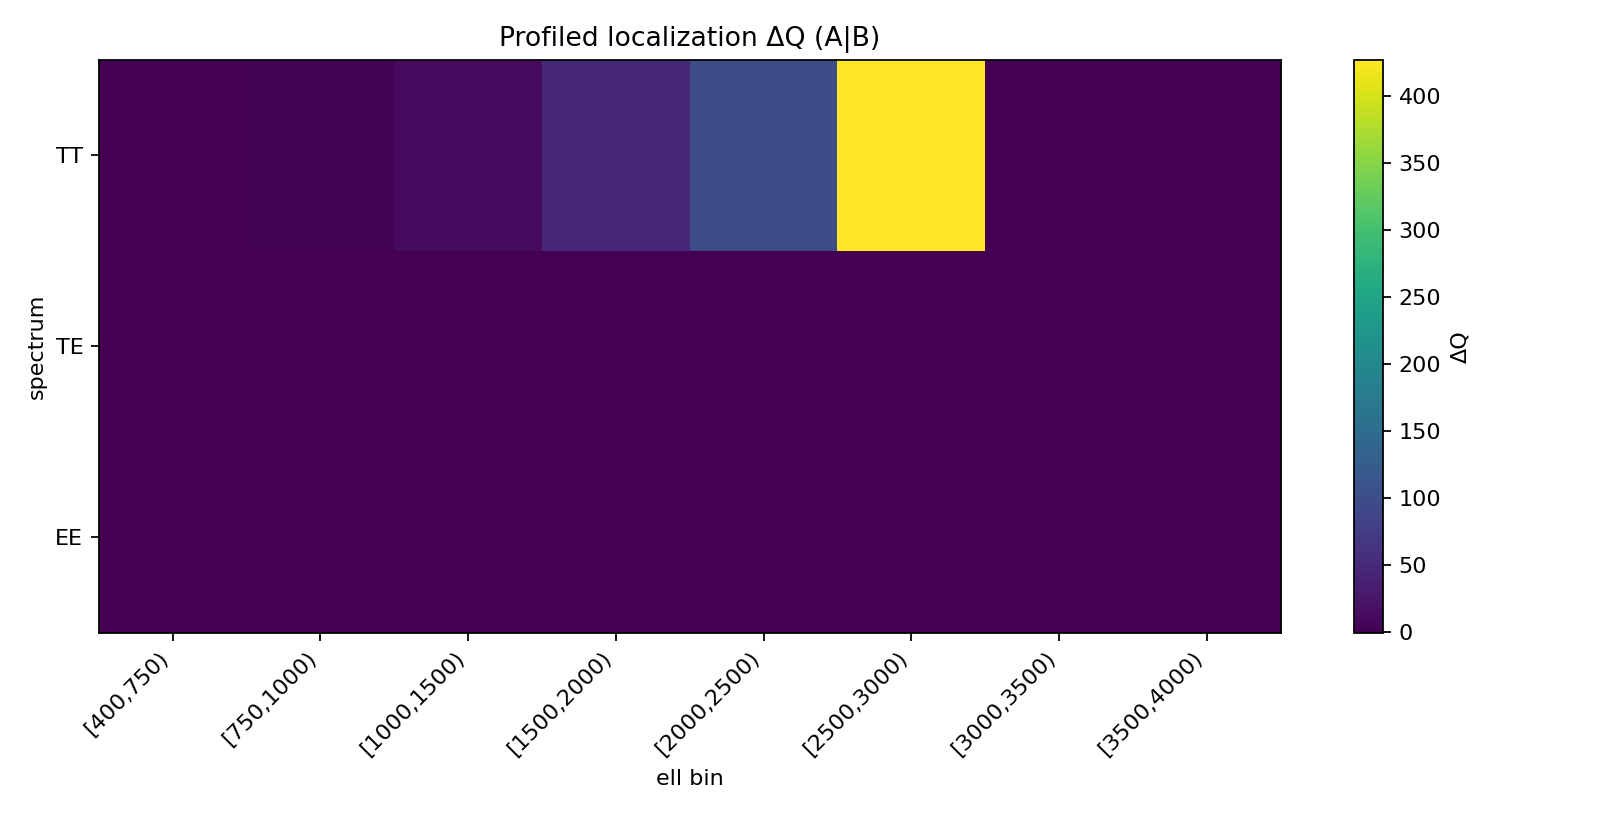
\includegraphics[width=0.49\linewidth]{figures/fig_profiled_localization_A_given_B.png}
  \caption{Profiled localization heatmaps for the SPT lens swap, decomposing the directional held-out mismatch into contributions grouped by spectrum type and multipole ranges. \textbf{Left:} $\dchi_{B|A}$ (SPT D1 given SPT2018). \textbf{Right:} $\dchi_{A|B}$ (SPT2018 given SPT D1). Darker regions indicate larger contributions to the held-out failure. In both directions, the dominant contributions arise from TT at high multipoles within the overlap region.}
  \label{fig:profiled-localization}
\end{figure}

\subsection{Common-staging changes mismatch only at the few-percent level}
A natural hypothesis is that the mismatch is driven by differences in multipole support between SPT2018 and D1. To test this, we implement a common-staging control in which the D1 lens is restricted (as much as feasible) to the SPT2018 multipole support and we repeat the same audits (\cref{sec:common-staging}).

Figure~\ref{fig:profiled-staging-compare} visualizes the baseline-vs-common-staging comparison for the \emph{profiled} audit. The resulting changes are modest: common-staging does not qualitatively resolve the mismatch, and the localization remains dominated by TT high-$\ell$ structure within the overlap region. This control therefore argues against a purely support/cut explanation for the lens mismatch and motivates treating parameter-level shifts (including $\mnu$ tightening) as packaging-sensitive unless accompanied by explicit lens-swap audits.

\begin{figure}[t]
  \centering
  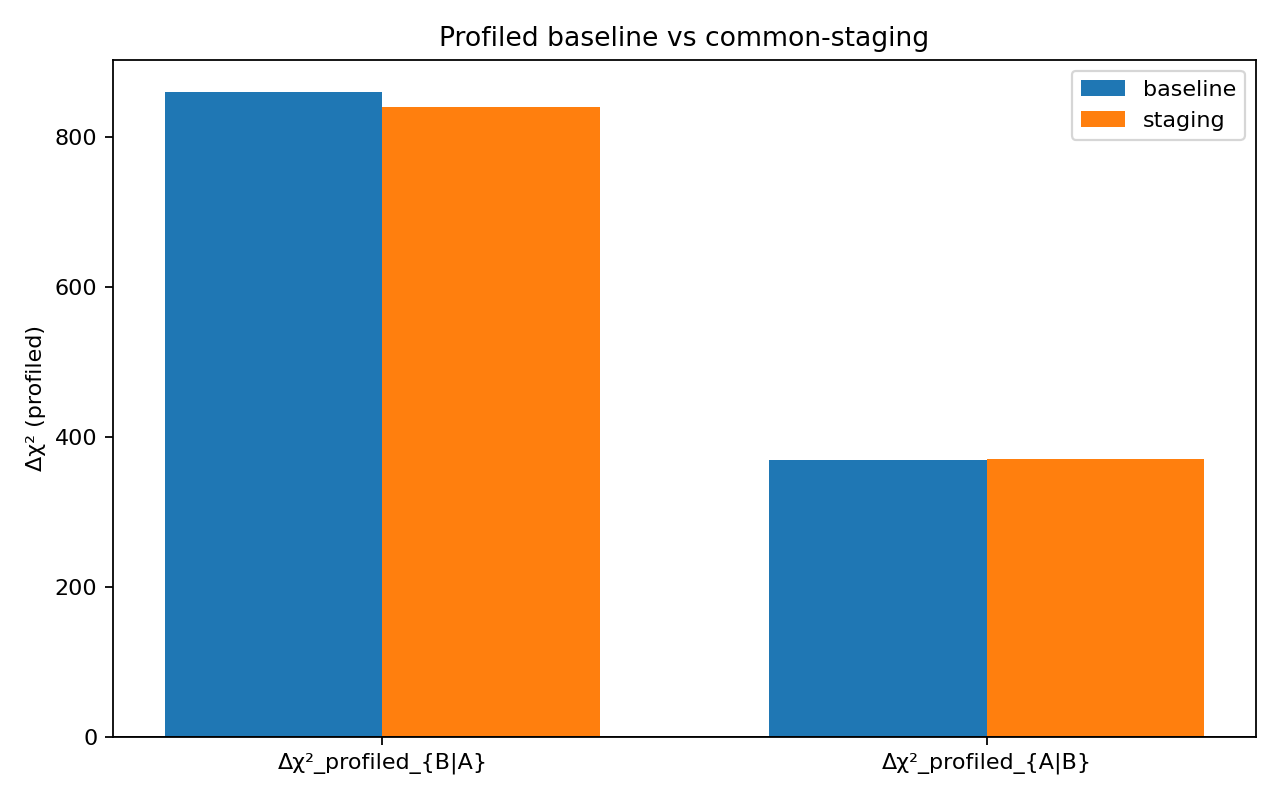
\includegraphics[width=0.85\linewidth]{figures/fig_profiled_staging_compare.png}
  \caption{Common-staging control for the profiled cross-lens audit. Baseline uses the full D1 multipole support; common-staging restricts D1 to the SPT2018 support. The change in $\dchi$ is small compared to the overall mismatch, indicating that staging alone does not explain the held-out failures.}
  \label{fig:profiled-staging-compare}
\end{figure}
